% Chapter Template

\chapter{\color{RoyalBlue!50!black} Neuronal Modulation Depends on Context and Feature Tuning} % Main chapter title

\label{ch:papernak} % Change X to a consecutive number; for referencing this chapter elsewhere, use \ref{ChapterX}

%----------------------------------------------------------------------------------------
%	SECTION 1
%----------------------------------------------------------------------------------------

\section*{Introduction}
The \gls{mt} area of monkey cerebral cortex is a well-studied extrastriate visual area known to have robust selectivity for visual motion features \parencite{Britten1992, Born2005, Pasternak2020}. Motion signals represented by the activity of neurons in this area are important for making memory-guided comparisons about visual motion direction \parencite{Lui2011, Wimmer2016, Katz2016}. Lesions of this area impair the ability to report whether the motion direction of a stimulus matched a previous example or not \parencite{Rudolph1999a, Bisley2000a}; whereas electrical stimulation of this area can bias the behavior of an animal as though a particular direction of motion was seen when in fact no direction information had been present \parencite{ Bisley2001, Salzman1992, Salzman1990}. These findings indicate a key role for \gls{mt} in representing behaviorally-relevant visual motion information, and demonstrate that \gls{mt} has an important role in task-related perceptual decisions. One open question, however, is how behavioral goals impact the neural activity in area \gls{mt} during sensory (e.g., encoding/decoding of stimulus) and non-sensory (e.g., reward contingencies, decision making, etc.) periods of the task.

Area \gls{mt} acts in concert with another brain area, the \gls{pfc}, in order to do memory-guided comparisons of motion direction. \Gls{pfc} and \gls{mt} are reciprocally connected \parencite{Ungerleider1986, Barbas1988, Petrides2006}, and both are involved in memory-guided motion comparison tasks \parencite{Zaksas2006}. Neurons in \gls{pfc} contain direction information during motion discrimination tasks, but this selectivity is largely attenuated when animals do not have to make perceptual decisions, or when that information is not relevant to the task \parencite{Hussar2009, Hussar2012, Hussar2013}. Previous research has also found reduced trial-to-trial variability in \gls{pfc} with increased task demands \parencite{Hussar2010}, suggesting \gls{pfc} neurons may be recruited to support task performance when needed. Because of the interconnected structural and functional relationship between \gls{pfc} and \gls{mt}, such a change in trial-to-trial \gls{pfc} variability with task demands may be reflected in \gls{mt} dynamics and altered processing of stimulus information, but this hypothesis remains untested.

To investigate this question, we measured how activity in \gls{mt} covaried with the differing demands of an active task and a passive task that used physically identical stimuli. The active task consisted of two random dot motion stimuli separated by a delay, where subjects (Rhesus macaques; \textit{Macaca mulatta}) had to report whether or not the direction of motion in the first stimulus (``\sample") matched the second (``\test''). During the passive task, no perceptual decision was required, but the motion stimuli were the same. Thus, despite practically identical sensory conditions, the task demands during active and passive tasks were different. Thus, the active task can be parsed as a sequence of: stimulus encoding (S1), memory maintainance (delay period), recall and comparison (S2), and finally decision making (S2/post-S2). For sensory periods (S1/S2), We hypothesized that heightened task demands during the active task would be reflected in sharper tuning, reduced trial-to-trial variability, and/or modulation gain, in line with prior findings about selective attention to motion direction \parencite{Trujillo2004, Ponce-Alvarez2013, Cohen2008, Arandia-Romero2016}. For the more cognitive aspects of the task (working memory, S1/S2 comparison signals, decision making), we expected to find stronger comparison effects, signals differentiating ``same" and ``different" trials independent of motion direction, in the active task. 

We found that the effects of heightened task demands depended on the amount of task-relevant stimulus information (e.g. direction selectivity) neurons conveyed. Specifically, we found three distinct modulation profiles for stimulus processing between the active and passive tasks: information-enhanced, information-suppressed, and \mbox{information-consistent} neurons. Neurons signalling enhanced task-relevant stimulus information during the active task displayed sharper tuning, and a preferential reduction in trial-to-trial variability, but no effect on comparison signals. In contrast, information-suppressed neurons displayed a flattening of their tuning curves with no effect of task on trial-to-trial variability. The third subpopulation of neurons (information-consistent), while significantly tuned to motion direction, displayed only weak effects of task on tuning or variability. Instead, the suppressed and consistent groups showed task-dependent comparison signals comparing S1 and S2. These results suggest a division of labor in area \gls{mt}, separating sensory processing and cognitive effects of the task across distinct subpopulations of neurons.

\section*{Results}
Three adult male Rhesus macaques (\textit{Macaca mulatta)} performed delayed visual motion comparison tasks while we recorded neural activity in MT (Figure \ref{fig:fig1}A). In the active task, monkeys indicated whether a second stimulus (``\test'') had the same or a 90-degree different direction of motion than a first stimulus (``\sample'') by making a saccade to one of two choice dots. All three monkeys performed above chance in the active task (m201, 10 sessions: $77.79\% \pm 1.08\%$ accuracy, m202, 28 sessions: $81.63\% \pm 0.95\%$, m317, 16 sessions: $85.77\% \pm 1.36\%$ ; $mean \pm Std$). The passive task, except for a different fixation point shape, was identical up to the choice window, at which time no choice target stimuli were shown and no further action was required to receive reward (Figure \ref{fig:fig1}A). 

\begin{figure}
	\centerline{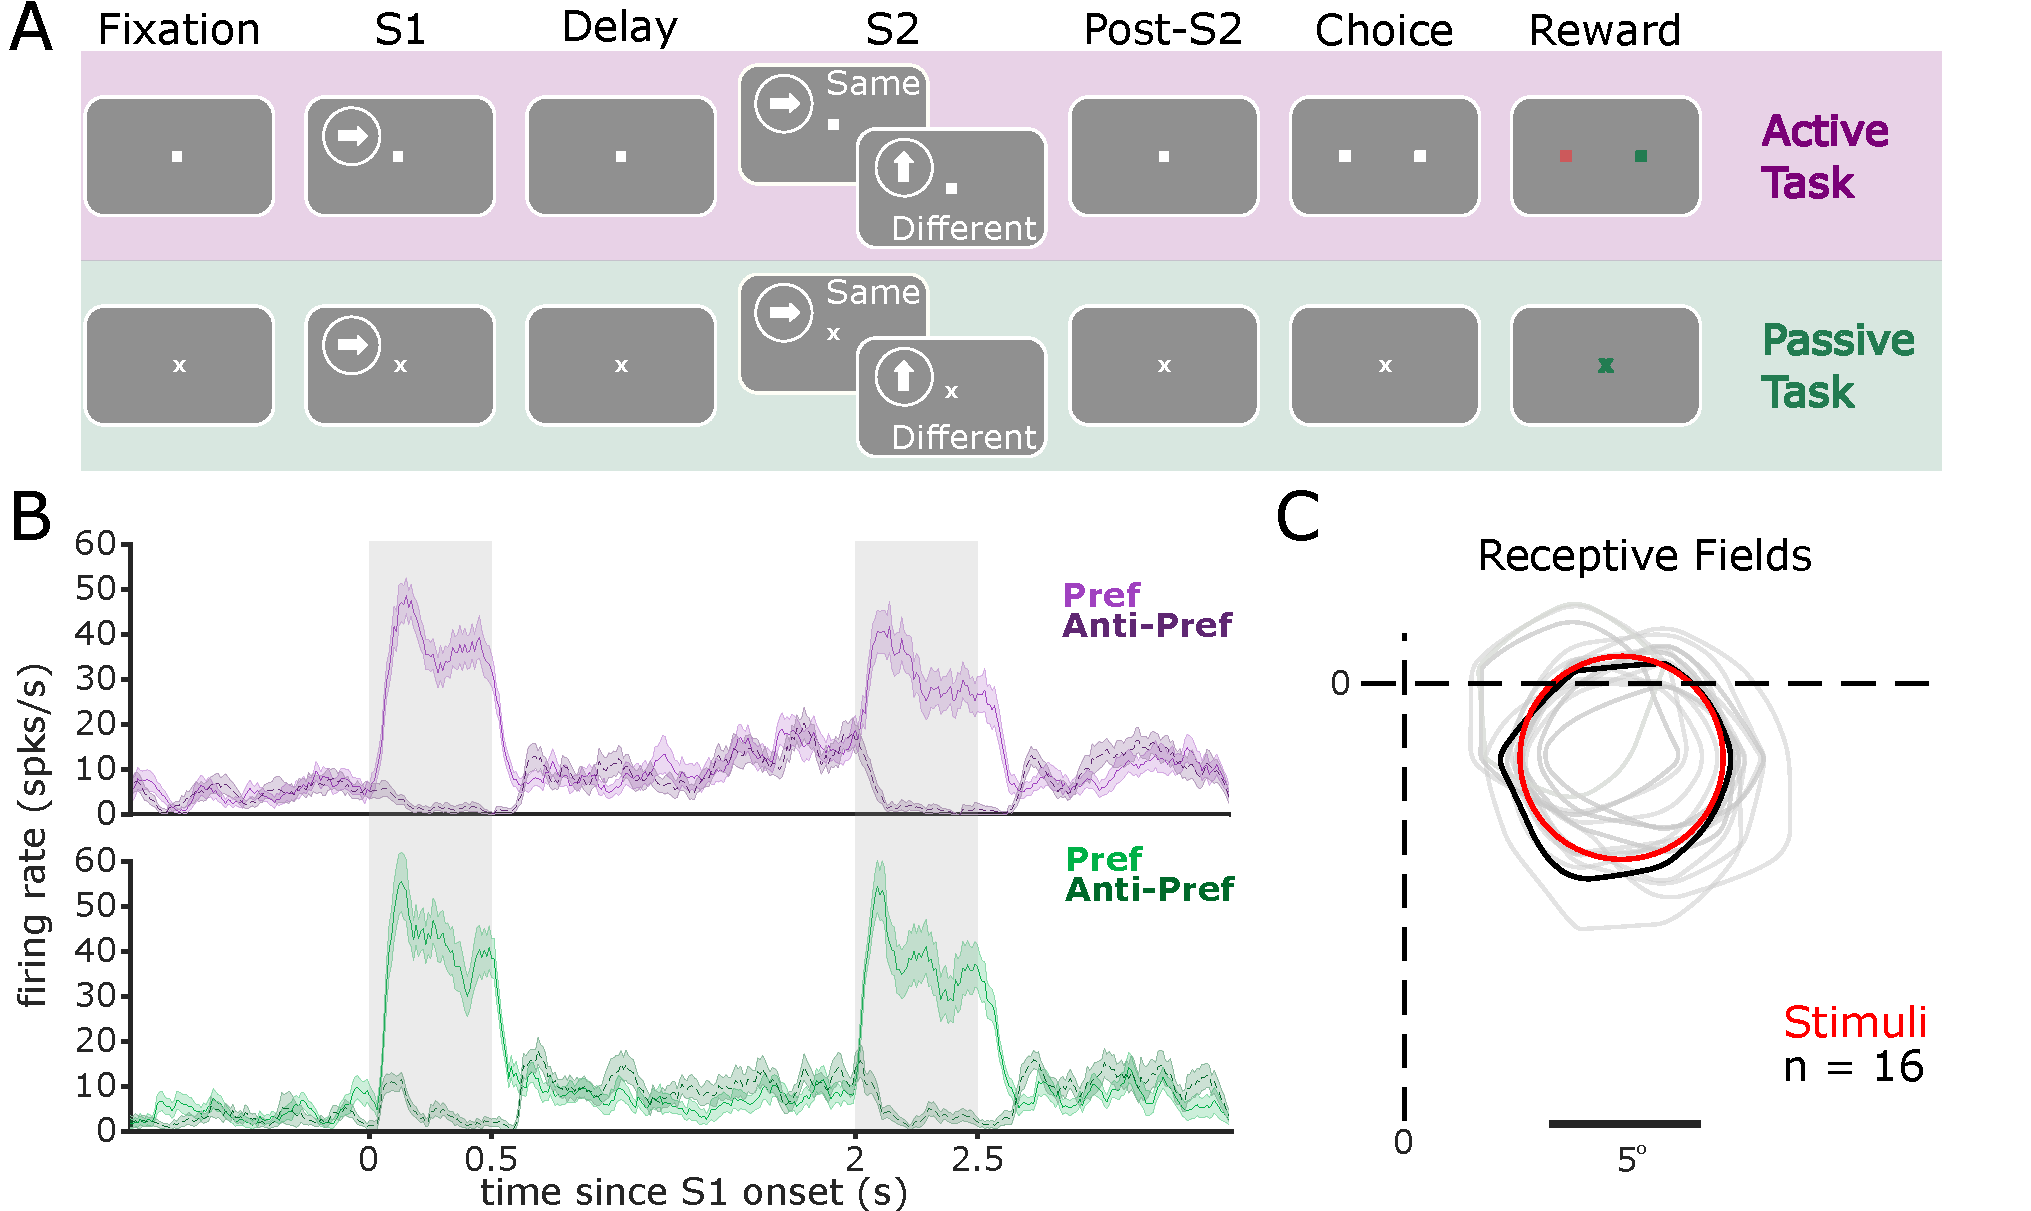
\includegraphics[width=172mm]{Figure1_taskEffects.pdf}}
	\caption{ \textit{Task design and task modulation of MT firing rates.} A. Trials consisted of a pre-stimulus fixation period, a first stimulus  (S1), followed by a 1.5 second delay, then a second stimulus (S2) and a post-S2 fixation period. After the post-S2 fixation period subjects were either rewarded (passive task) or had to report a decision with a saccade and rewarded after correct choices (active task). Stimuli moved in one of 8 directions ($0^\circ$, $45^\circ$, $90^\circ$, $135^\circ$, $180^\circ$, $225^\circ$, $270^\circ$, $315^\circ$) during S1, and then S2 was either in the same direction, or $90^\circ$ off of S1 (rotated left or right). B. PSTHs of an example neuron that was recorded in both tasks. Solid line represents the neuron’s response to its preferred motion direction while dashed lines indicate $180^\circ$ away from preferred (“anti-preferred”) C. Receptive fields (grey) of each simultaneously-recorded neuron from one example session, along with the location and size of the stimuli (red). Black curve corresponds to example neuron in B. Contours represent isointensity responses at $50\%$ of the peak response. }
	\captionsetup{singlelinecheck = false, font=footnotesize, labelsep=space, width=172mm}
	\label{fig:fig1}
\end{figure}

Neurons were recorded with receptive field centers of $10.55 \pm 0.77$ Degrees of visual angle eccentricity ($mean \pm SEM$ across all neurons from all sessions; Figure \ref{fig:fig1}C for example session). Neurons were included for analysis if: 1.) Their 50\% isointensity response field (see \hyperref[{sec:methods}]{Methods}) was at least 30\% covered by the stimuli, 2.) the subject did at least 10 trials in each direction condition, and 3.) they were confidently recorded across both tasks (see \hyperref[{sec:methods}]{Methods}). This resulted in 254 well-defined neurons included for analysis. 

We were interested in the impact of cognitive demands on \gls{mt} activity. Such demands varied over the course of a trial in the active task, including periods where stimuli were present (i.e., during \sample\ and \test) and also periods where stimuli were absent (i.e., pre-\sample, the delay, and post-\test). For example, prior to \sample, the animal should prepare cognitive resources in anticipation of the stimulus. Then, during \sample, the animal must process and store task-relevant information (motion direction). During the delay, this information must then be maintained in working memory and the appearance of \test\ may be anticipated. During \test, task-relevant information must again be encoded, the stored information about \sample\ retrieved, and a comparison judgement made. These dynamic task demands may result in varying effects on \gls{mt} activity across these different stages. We first describe the effect of task demands on motion-direction signalling by \gls{mt} activity during stimulus presentations (\sample\ and \test).
Second, we will describe effects of task demands on \gls{mt} activity when stimuli were absent. Third, we will describe effects of task demands on \gls{mt} activity during the comparison stage of the task (\test\ through decision).

\glsreset{mi}
\subsection*{Task effects in MT depend on neural tuning}
We hypothesized that the accuracy of motion direction encoding in \gls{mt} would improve when that information was task-relevant (i.e., in the active task compared to the passive task).
To test this, we measured the \gls{mi} between neural firing rates and the motion direction of \sample\ and \test. \Gls{mi} quantifies how much information about one signal is provided by another signal (and vice-versa), and takes into account both the tuning of neural responses with respect to a stimulus as well as trial-to-trial response variability (\cite{Hatsopoulos1998, QuianQuiroga2009}; see \hyperref[{sec:methods}]{Methods}).
Across all neurons in our sample, we found similar degrees of motion direction signalling in the active and passive tasks (Figure \ref{fig:MI}A). As \gls{mt} is a mid-level sensory area, this was unsurprising. 

\begin{figure}
	\centering
	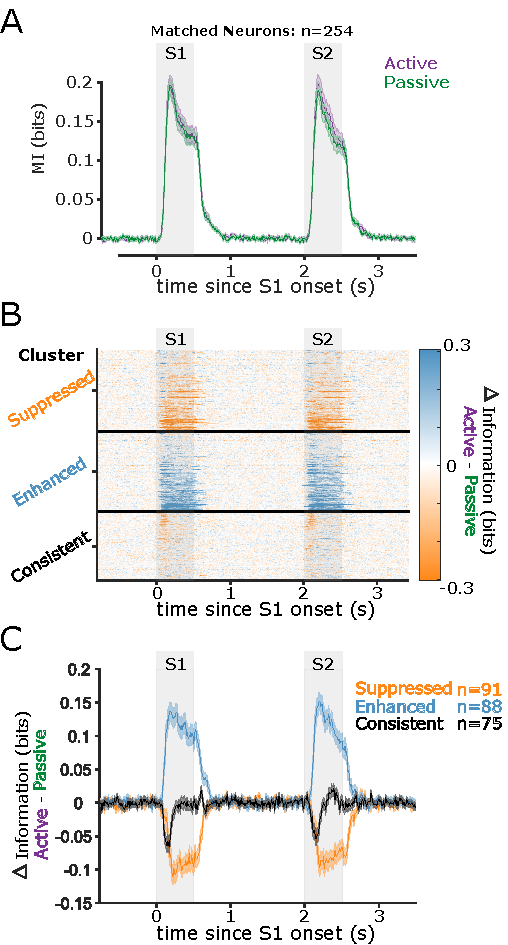
\includegraphics[width=86mm]{ClusteringFigMatched.pdf}
	\caption[Unsupervised Clustering of neurons by Task-Effect]
	{{\it Motion Information Clustering.} A.) Time course of mutual information between matched neurons firing rates' and motion direction in the active and passive task. B.) Time series for active minus passive motion information (\gls{mi}) within neuron. Each row is a single neuron matched across task, and color represents the difference in information. See \hyperref[{sec:methods}]{Methods} for clustering algorithm. C.) Within-cluster averages from panel B.}
	\captionsetup{singlelinecheck = false, font=footnotesize, labelsep=space}
	\label{fig:MI}
\end{figure}

We hypothesized that changing task demands might be especially impactful on the activity of neurons that signal task-relevant information.
That is, switching from passive viewing to a task requiring judgment of motion direction might have a particularly strong effect on neurons strongly signaling motion direction compared to neurons that did not signal that information so strongly.
To test this hypothesis, we calculated the task effect of motion information for each neuron by subtracting the timeseries during the passive task from the active task. This provided a metric which quantifies, at each timepoint, how each neuron signals motion direction information differently across tasks (Figure \ref{fig:MI}B). We then clustered neurons according to the Pearson distances between these task effect time-courses (see \hyperref[{sec:methods}]{Methods}). We found 3 clusters to be the most parsimonious model, and hereby refer to them as suppressed, enhanced, and consistent groups (Figure \ref{fig:MI}B\&C), which describes the average task effect on direction information for neurons within each cluster.

% not sure how/if to include this information
%($1 Cluster: BIC=1.191, 2 Clusters: BIC=1.206, 3 Clusters: BIC=0.941, 4 Clusters: BIC=1.020, 5 Clusters: BIC=1.091$)

We found it interesting that a substantial group of neurons displayed a marked reduction in \gls{mi} during the active task (suppressed), as it represents a detriment in the population of neurons for direction coding. Taken together with the enhanced neurons, which followed the expected pattern of improved direction signalling, these results suggest that heightened task demands result in task-relevant information becoming disproportionately represented in a smaller number of highly-informative neurons.

%\subsection*{\color{rouge} Heightened Task Demands Flatten the Tuning Curves of Less-relevant Neurons}
\subsection*{Heightened Task Demands Differently Impact Tuning for Subpopulations of Neurons}
We found that mutual information between neuron firing rates and motion direction changed when motion direction was task-relevant (active task) compared to when it was not (passive task). Since \gls{mi} takes into account both stimulus tuning and trial-to-trial variability, the observed changes in \gls{mi} could be consistent with a change in tuning, a change in trial-to-trial variability, or a mixture of both. To better characterize the nature of the task-demand effects we found, we separately analyzed tuning and trial-to-trial variability for enhanced, suppressed, and consistent neuron groups.

\begin{figure}
	\centering
	\captionsetup{singlelinecheck = false, font=footnotesize, labelsep=space}
	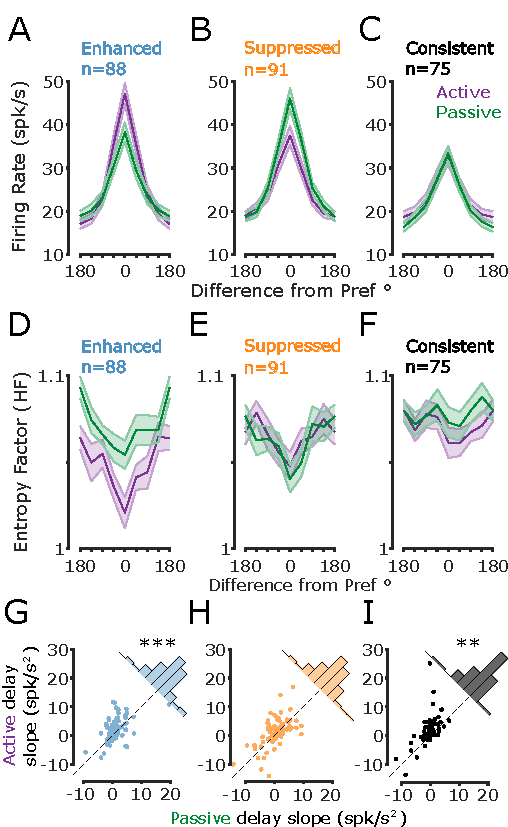
\includegraphics[width=86mm]{tuningAndHFmatched.pdf}
	\caption{{\it Effects of task demands differed depending on how informative a neuron was about task-relevant information.} A.) Average Tuning Curves for information-enhanced neurons during the active (purple) and passive (green) tasks. Both curves contain the same neurons. Error bars are $\pm SEM$ across neurons.B-C.) Same as A for information-suppressed and consistent groups respectively. D.) Average trial-to-trial variability during S1 quantified with \gls{hf} (See \hyperref[{sec:methods}]{Methods}). E-F.) Same as panel D for information-suppressed neurons and consistent groups respectively. G.) Slope of a linear fit to enhanced neurons' firing rates vs time during a 1s interval before S2 onset in the Active vs Passive tasks. There was a significantly higher ramping during the active task (***: $p=5.66\cdot10^{-5}$, t-test). H-I.) Same as panel G for information suppressed (ns) and consistent (**: $p=0.0098$) groups respectively.}
	\label{fig:interaction}
\end{figure}

We tested for differences in tuning for each group by calculating the average firing rate for each neuron, and compared effects of task, direction condition, and stimulus (3-way ANOVA: Figure \ref{fig:interaction}A-C). The main effect of `stimulus' (S1 vs S2) was negligible for each group (enhanced: $p=0.238$; suppressed: $p=0.187$; consistent: $p=0.531$), so for visualization purposes we plotted S1, which unlike S2 does not have concurrent comparison processes. We found the expected pattern of tuning modulation for enhanced neurons, with gain around preferred direction and suppression to 180 degrees off preferred, supported by an interaction effect between task and direction ($p \approx 0$: Figure \ref{fig:interaction}A). In contrast, the information-suppressed group showed a reduction in response around their preferred stimulus in the active task (Figure \ref{fig:interaction}B). Interestingly, the consistent group shows a slight increase in response to anti-preferred motion (180deg off pref) which results in a flattening of their tuning curves (task effect: $p=0.005$). This means that during the active task, neurons that had suppressed or consistent information  had flatter (broader) tuning profiles, which in isolation would constitute a deficit to direction coding when that information is task-relevant.

\glsreset{hf}
\subsection*{Trial-to-Trial Response Variability is Modulated by task and Stimulus Features}
In addition to tuning, \gls{mi} also takes into consideration trial-to-trial variability in responses. we reasoned that the task effects on \gls{mi} may be partially due to altered variability of neural responses. To test this, we calculated the entropy of neural responses (separated again by task, motion direction, and stimulus, 3-way ANOVA) and normalized measurements relative to those of a simulated Poisson process matched for intensity (\gls{hf}; see \hyperref[{sec:methods}]{Methods}).

We found an overall reduction in \gls{hf} in the active task, relative to the passive task for information-enhanced neurons ($F=60.24, p \approx 0$; Figure \ref{fig:interaction}D). Additionally, all three classes of neurons had a reduction in trial-to-trial variability that was a function of motion direction (enhanced: $F=6.64$, $p \approx 0$; suppressed: $F=6.97$, $p \approx 0$; consistent: $F=2.07$, $p=0.044$; Figure \ref{fig:interaction}D-F). Neurons had the largest reduction in \gls{hf} to their preferred stimuli, with weaker effects as motion direction diverged from this direction. The preferential reduction in variability was strongest in the information-enhanced group, consistent with the improvement to both tuning and \gls{mi}. No active vs. passive task effect was found for the information-suppressed group, though they did still display an effect of motion direction on \gls{hf} that was consistent with the enhanced neurons. Information-consistent neurons showed a weak improvement in \gls{hf} that likely counteracted the weak detriment in tuning, resulting in the net zero change in motion direction information that classifies the group.

To summarize, all three groups of information-modulated neurons displayed different patterns of tuning and variability modulation, which further supports our hypothesis that these groups of neurons differently contribute to the task.


\subsection*{Task Demands Modulate MT Firing Rates During Non-stimulus Periods}
We next turned our attention to the effects of varying task demands on \gls{mt} activity during periods when dot motion stimuli were absent (pre-\sample, during the delay between \sample\ and \test, and post-\test). Because no stimuli were present, effects during these intervals would be due only to cognitive processes (e.g., anticipation of \sample\ or maintenance of memoranda during the delay).
The pre-S1 period was highly predictable in this task (1000ms post fixation), so we expected to see a gradual increase (``ramping'') of firing rate during this period, reflecting anticipation. We quantified pre-\sample\ ramping as the slope of a linear fit to FR vs. time during a one second window before \sample\ onset. We found a significant task effect of pre-\sample\ ramping only within the information enhanced group (T-test Passive minus Active slopes: $p=1.02\cdot 10^{-4}$).

Next we considered the delay period between \sample\ and \test. Because the timing of this delay was also highly predictable in our task (always 1.5 seconds), animals could anticipate the appearance of \test. We also found significant ramping during the delay period for enhanced neurons ($p=5.66\cdot10^{-5}$) and consistent neurons ($p=0.0098$), where both groups had higher delay ramping in the active task (Figure \ref{fig:interaction}G-I).  This increased ramping in the active task may reflect additional task demands related to the preparation of the \sample\ and \test\ comparison.
We also asked whether \gls{mt} activity might continue to be selective for the motion direction of \sample\ during the delay, which could be consistent with a working-memory-related maintenance process. However, we found that \gls{mi} between \gls{mt} activity and \sample\ motion direction rapidly fell to levels consistent with the null hypothesis after \sample\ offset, and this did not differ based on task demands (Figure \ref{fig:MI}A).

\subsection*{MT Activity is Affected by Cognitive Aspects of Memory-guided Visual Comparisons}
During \test\ of a given motion direction, our active task required subjects to make a saccade to the right if the direction of the preceding \sample\ was the same (``same trial''), and a saccade to the left if the direction of the preceding \sample\ was different (``different trial'').
It has previously been observed that \gls{mt} neurons' responses to physically identical \test\ stimuli differed whether they came from ``same'' or ``different'' trials, which we termed a ``comparison effect'' \parencite{Lui2011,Zaksas2006}. 
Here we ask: (1) are CEs different in the active versus the passive task (when no comparison is needed); and (2) is the task-modulation of CEs (if any) different across the three neuron groups (enhanced, suppressed, consistent)?

\begin{figure}
	\centerline{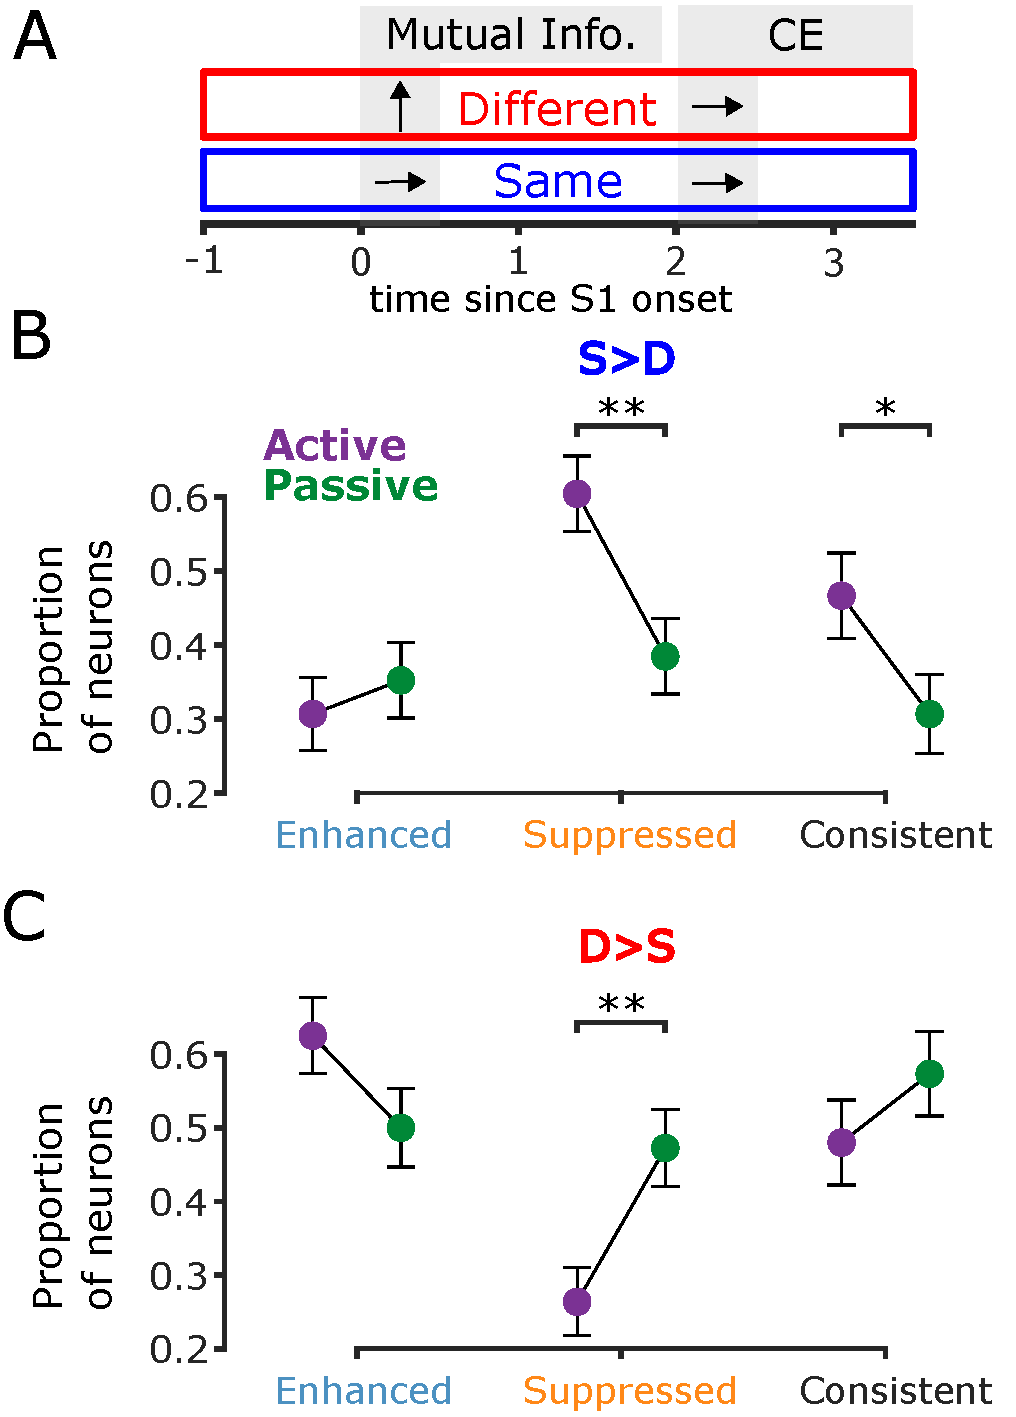
\includegraphics[width=86mm]{CEproportions.pdf}}
	\caption{\textit{Recruitment of MT neurons for cognitive aspects of the task} A.) Schematic of comparison effect analyses. Neurons were classified into groups according to their Pearson distance during S1 and the Delay. Comparison effects were then calculated from S2 onset up to the appearance of the choice targets. B.) Proportion of neurons within each information group with significant $S>D$ signal at some point during the CE window in panel A. C.) Same as panel B for $D>S$ neurons.}
	\label{fig:CEproportions}
\end{figure}

We calculated comparison effects as the area under the receiver operating characteristics curve (AUC) within direction condition during \test, between ``same'' and ``different'' trials (Figure \ref{fig:CEproportions}A). We expected that the cognitive effects of the task may run orthogonal to the sensory improvements (i.e. stronger comparison effects in non-enhanced groups), and this would be indicative of a division of labor. We indeed found that information-suppressed and consistent groups showed a significant increase in the number of $S>D$ neurons with no effect in the information-enhanced group (Figure \ref{fig:CEproportions}B; Suppressed: $\chi^2=8.79, p=0.003$, Consistent: $\chi^2=4.05, p=0.044$). Interestingly, the suppressed group show a reduction in $D>S$ neurons in the active task (Figure \ref{fig:CEproportions}C; Suppressed: $\chi^2=8.53, p=0.0035$). An important point to note here, is that the same proportion of significant neurons in all three information groups shows CEs during the passive task, and the active task influenced their cognitive contributions differently. 

\begin{figure}	
	\centering
	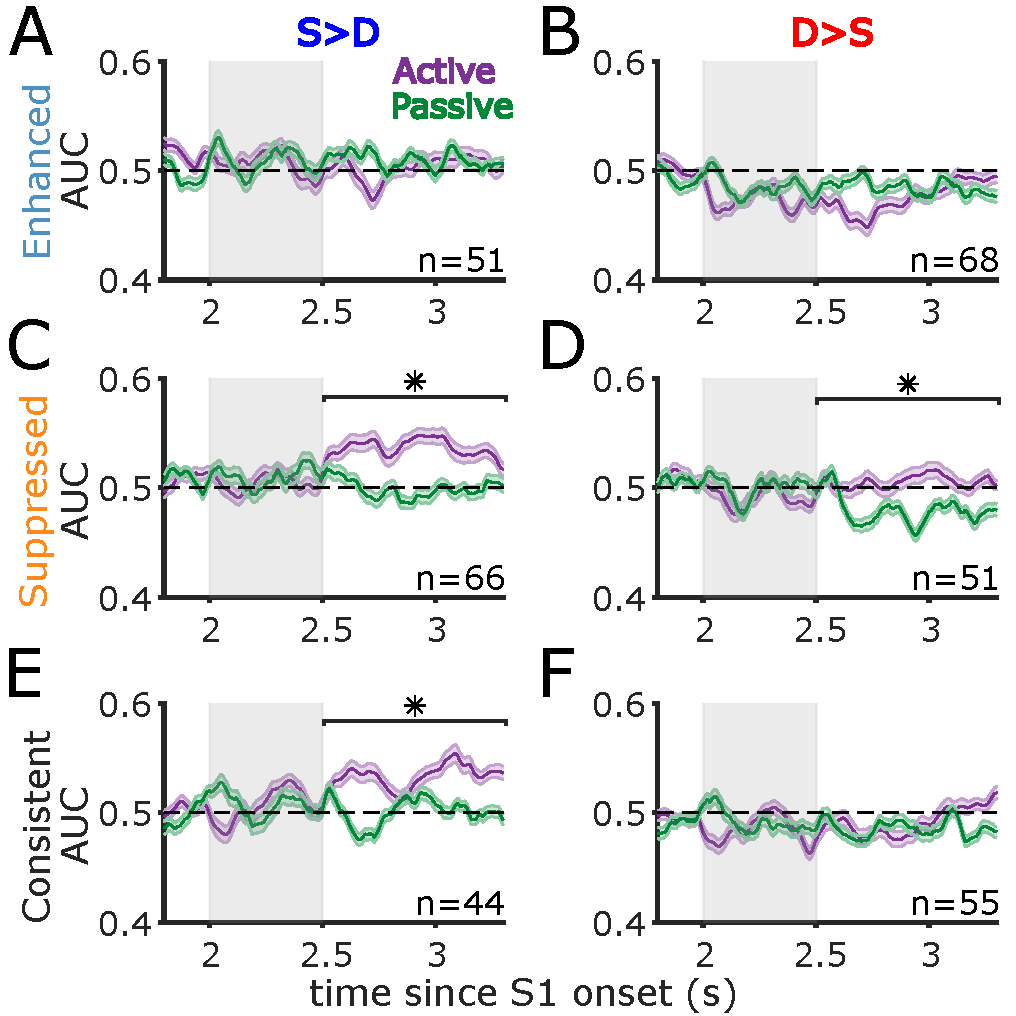
\includegraphics[width=86mm]{CEtimecourses.pdf}
	\caption{\textit{Comparison Effects increase from stimulus to decision} A.) Time course of comparison effects (AUC between same and different trials within stimulus type) for neurons that were information-enhanced and significantly $S>D$ in either task. B.) Same as panel A but for information-enhanced $D>S$ neurons. C-D.) Same as A-B but for information-suppressed neurons. E-F.) Same as A-B but for information-consistent neurons. *: $p<0.05$ for the difference between tasks over the indicated interval.}
	\label{fig:CEtimecourses}
\end{figure}

We next looked at the time courses of comparison effects from S2 through appearance of the choice dots (Figure \ref{fig:CEtimecourses}), again separated by information-group and direction of CE. These time courses reflect the aforementioned division of labor, where the information-suppressed and consistent groups contribute to the cognitive aspects of the memory-guided comparison (Figure \ref{fig:CEtimecourses}C-F), while the information-enhanced group does not (\ref{fig:CEtimecourses}A-B). So, in addition to a higher proportion of neurons signalling CEs, the average CE signal ($S>D$) during the post-S2 window also increased with heightened task demands (Figure \ref{fig:CEtimecourses}C \kst\ test: $p=1.11 \cdot 10^{-5}$; Figure \ref{fig:CEtimecourses}E \kst\ test: $p=8.22 \cdot 10^{-4}$). The higher proportion of $S>D$ neurons in the suppressed and consistent groups, along with their increased CE signalling, indicates that while these groups did not improve stimulus encoding with heightened task demands, they were recruited to aid with the comparison of S1 and S2. 


\section*{Discussion}
\glsresetall
We hypothesized that neurons in the primate \gls{mt} area behave differently when task demands increase in order to improve information processing for goal-oriented behavior. We tested this hypothesis by recording activity of \gls{mt} neurons in monkeys performing two tasks, one active and one passive.
We found that in the active compared to the passive task, (1) three patterns of task effects on information signalling arose that were distributed across subpopulations of neurons, and (2) sensory and cognitive aspects of the tasks are handled separately by these subpopulations.

We found that firing rates of neurons in \gls{mt} contained direction information during the stimulus periods (Figure \ref{fig:MI}A), and that increasing task demands had one of three broad effects on motion information for each neuron: information-enhancement, information-suppression, or information-consistent effects (Figure \ref{fig:MI}B). We then asked whether the changes in \gls{mi} were caused by tuning or variability. However, the extent to which tuning and variability are each influenced by cognitive factors has been a subject of intense research \parencite{Renart2014,Gilbert2013}, and each has different implications for computation and neural mechanisms. To better characterize the role of task demands on motion direction signaling in \gls{mt} in the context of this prior work, we separately examined tuning and variability. As the neurons were matched across task, we could directly compare how each neuron responded to motion in the active and passive conditions. Information-enhanced neurons showed sharper tuning curves with larger responses to their preferred motion direction and a suppression to anti-preferred (Figure \ref{fig:interaction}A). Information-suppressed neurons on the other hand, displayed a marked reduction in response to their preferred stimulus in the active task, resulting in the detriment to \gls{mi} observed. As a result, these neurons became less tuned for motion direction when that information was more task-relevant. These effects on tuning are consistent with the classification of neurons based on changes to motion direction signalling in \gls{mi}, but may not account for the full picture, as \gls{mi} is also affected by trial-to-trial response variability, which we examined next. 

By measuring \gls{hf}, we found a strong relationship between direction preference and variability, which did not depend on group (Figure \ref{fig:interaction}D-F). Neurons had the largest reduction in trial-to-trial variability during presentations of their preferred stimulus, with weaker effects as direction diverged from preferred. This cannot be due to the increased firing rate for those directions, as \gls{hf} accounts for rate effects (see section \hyperref[{sec:methods}]{Methods}), and a rate confound would result in the opposite trend (that is, typically variability is biased downward for lower rates, but we found higher variability at lower rates; \cite{Churchland2010}). The effect of heightened task-demands in the active task was largest for the information-enhanced neurons, which compound the tuning-based improvements to \gls{mi} (Figure \ref{fig:interaction}D). Interestingly, suppressed neurons showed no effect of task on variability, whilst maintaining the effect of motion direction. This means that heightened task demands flatten the tuning curves of these neurons, without altering the trial-to-trial variability.
Previous researchers have suggested that a substantial portion of trial-to-trial variability can be understood in terms of neurons' susceptibility to changes in cognitive state \parencite{Ecker2016a,Denfield2018a}; thus one interpretation of this pattern of results is that these neurons decrease their participation in sensory processes (reduced tuning) while maintaining their participation in more cognitive processes (consistent trial-to-trial variability)
The reduction in trial-to-trial stimulus response variability we observed in enhanced neurons when task demands were elevated is reminiscent of the finding of \textcite{Mitchell2007}, who found general reductions in Fano Factor in V4 responses when animals selectively attended to a stimulus compared to when that stimulus was not attended.
The novel and more surprising result we found is that the strength of variability reduction depended on whether the stimulus was preferred (great reduction in variability) or less-preferred (less reduction in variability). This suggests that one effect of elevating task demands is a preferential improvement to information transmission reliability according to neurons' feature tuning.

We found significant changes in non-stimulus firing rate (FR) in the active task compared to the passive task, such as larger FR ramping during the delay period (Figure \ref{fig:interaction}G-I). Ramping of neural firing rates has traditionally been explored in the context of motor preparation \parencite{Ding2015, Narayanan2016}, and decision making \parencite{Shadlen2001}, where it has been typically linked to anticipation. Finding anticipatory increases in firing rate for sensory neurons in MT is interesting, and is not likely explained during the pre-\test\ interval of our tasks through either decision making or motor planning, as neither a correct decision or appropriate motor plan can be made before first seeing \test . 
More likely, the ramping we observed is related to preparing cognitive and attentional resources for the perceptual phases of the task, which had highly predictable timing, as has also been found for LPFC neurons \parencite{Hussar2010, Bisley2004}. This line of thought has also been explored in the context of another nearby visual region, V4 \parencite{Snyder2018,Luck1997}, where anticipatory ramping has been linked to interactions between V4 and prefrontal cortex \parencite{Snyder2021}. 
Taken together, these results suggest anticipatory signals may originate in prefrontal cortex and influence visual cortex via top-down feedback.

In addition to the more strictly sensory aspects of the task, the active task contains a comparison component which requires additional cognitive resources such as working memory. 
A greater response to \test\ on ``different'' trials compared to same trials (``$D>S$'') could be consistent with a response adaptation effect, while a greater response to \test\ on ``same'' trials (``$S>D$'') would be more consistent with a facilitation effect \parencite{Kohn2003}. We would expect that if CEs in \gls{mt} are explained primarily by adaptation/facilitation, we should find similar effects in the active and passive tasks; any task effect should indicate a greater role for memory-guided comparison processes.
We found no difference in comparison effects for information-enhanced neurons but significantly more extreme comparison effects for the suppressed and consistent groups (Figure \ref{fig:CEtimecourses}).
These cognitive effects being isolated to neurons that became worse at signalling motion direction when that information became more task-relevant further supports a division of labor in area MT for completing the task.
We found that comparison effects emerged most clearly during the period after the offset of \test\ and before the execution of the response saccade (the `post-\test' interval). 
This underscores the non-sensory, cognitive nature of these effects (since the sensory stimulus was absent when effects were strongest), and reduces the potential that response adaptation or repetition suppression could explain D$>$S comparison effects \parencite{Lui2011,Kohn2003}.
This relatively late time-course of comparison effects in \gls{mt} differs from earlier reports, which found comparison effects emerging shortly after \test-onset \parencite{Lui2011,Zaksas2006}. 
One reasonable explanation for this difference in the timing of comparison effects across studies is the difference in timing between the onset of \test\ and the animals' reports. 
Earlier studies required the animals to respond immediately following the offset of the \test, whereas in the current study animals must withhold responding until after the post-\test\ delay. 
Thus, if the timing of comparison effects was more tightly related to the animals' reports than to the time of \test\ onset, then that would be consistent with the results across all these studies of comparison effects in \gls{mt} and further underscores the cognitive role of comparison signals.
Finally, in earlier studies decisions were reported with a manual button press \parencite{Lui2011,Zaksas2006}, whereas the current study required animals to report with a saccade, reinforcing the notion that comparison effects are related to cognitive decisions rather than the formation of particular motor plans.
\begin{center}
	\begin{table*}
		\begin{tabular}{|c|c|c|c|c|c|c|c|c|}
			\hline
			\textbf{Class} & \multicolumn{3}{|c|}{\textbf{Tuning}} & \multicolumn{3}{|c|}{\textbf{HF}} & \textbf{Delay Ramping} & \textbf{CE} \\
			\cline{2-7}
			& Task & Dir. & Stim. & Task & Dir. & Stim. &  &  \\
			\hline
			\textbf{\textcolor{enhanced}{Enhanced}} & *** & *** & ns  & *** & *** & * & *** & ns \\
			\textbf{\textcolor{suppressed}{Suppressed}} & *** & *** & ns & ns & ** & * & ns & ** \\
			\textbf{Consistent} & ** & *** & ns & ** & * & * & ** & * \\
			\hline
		\end{tabular}
		\caption{Task effects summary. Significance of task effects separated by information clusters (*: $p<0.05$, **: $p<0.01$, ***: $p<0.0001$, ns: not significant). Statistics for Tuning and entropy (HF) were a three-way anova between task, motion direction, and stimulus (S1 vs. S2). Comparison Effects (CE) were $\chi^2$ tests between the active and passive tasks (\ref{fig:CEproportions}B). Delay ramping was compared using t-tests on the slopes (Passive minus active: (\ref{fig:interaction} G-I).}
	\end{table*}
\end{center}

\subsection*{Conclusion}
In the present study, we investigated the effects of task demands on information processing in area MT of the macaque. We found substantial differences in variability and tuning profiles depending on the degree to which a neuron represented task-relevant information in its firing rate. In addition to these sensory components of the task, MT neurons also show stronger cognitive signalling with heightened task demands, such as anticipatory ramping and heightened comparison effects. These results highlight the role of MT populations in all phases of memory-guided comparisons of visual motion direction, and, combined with the previous findings in \gls{pfc}, suggest a continual interplay between prefrontal and extrastriate visual cortical areas during cognitive task performance. Importantly, involvement in sensory versus cognitive processes was found to be flexibly distributed across subpopulations of \gls{mt} neurons, with some neurons taking on greater sensory signaling when task-relevant, and other neurons shedding sensory selectivity in seeming favor of greater cognitive responsibilities.



\section*{Methods}
\label{sec:methods}

\subsection*{Resource Availability}
\subsubsection*{Lead Contact }
Requests for further information should be directed to the lead contact Adam Snyder (adam.snyder@rochester.edu).

\subsubsection*{Materials Availability }
This study did not generate any new reagents. 

\subsubsection*{Data and Code Availability}
Data and code used for this paper are made available by request through the lead contact.

\subsection*{Subjects} 
Subjects used in this study were three adult male rhesus macaques ages 7, 8, and 7 years, for 201, 202, and 317. All training, surgery, and experimental procedures were performed in accordance with the National Institutes of Health \textit{Guide for the Care and Use of Laboratory Animals} and were approved by the University of Rochester Committee for Animal Research. Surgery was performed using aseptic technique with isofluorane general anesthesia and perioperative opiate analgesics. An initial surgery was performed to implant a surgical steel head holder restraint embedded in bone cement secured to the cranium with ceramic bone screws. After behavioral training, a subsequent surgery was performed to implant a PEAK canula (19 mm diameter; Crist Instruments, Hagerstown, MD) over MT.

\subsection*{Data Acquisition} 
Recording chambers enclosed the craniotomies and contained 1mm-spaced CILUX grids (Crist Instruments). Thirty-two-channel S-probes (Plexon, Dallas Texas) were lowered through custom-made steel guide tubes, which were themselves inserted just low enough to penetrate the dura. We then drove the electrodes using a NAN electrode drive (NAN Instruments, Nof Hagalil, Israel). Recordings were done by coordinating a Plexon (Dallas, Texas) Multichannel Acquisition Processor and the data acquisition system TEMPO (Reflective Computing).

\subsection*{Receptive Field Mapping}
Prior to each recording session, receptive fields were mapped in order to identify where the stimuli should be displayed. The initial manual phase consisted of moving a patch of dot motion around on the stimulus display with a computer mouse while listening to spiking activity via an audio monitor. Afterwards, we presented small dot motion patches ($1^{\circ}$) in different directions on the vertices of a grid spanning the likely RF area identified in the manual step. Stimuli for each session were placed such that they covered the aggregate receptive field area for the recording (Figure \ref{fig:fig1}B).

\subsection*{Stimulus Presentation}
Stimuli were presented at 75 Hz monitor refresh rate on a 19-inch IIyama Vision Master Pro-513 monitor with 1,152 by 870 pixel resolution. They were $100\%$ motion-coherence random dot kinematograms in one of 8 directions ($0^\circ, 45^\circ, 90^\circ, 135^\circ, 180^\circ, 225^\circ, 270^\circ, 315^\circ$) placed in a circular aperture fit to the size of the receptive fields, with a dot diameter of $0.03^{\circ}$ and a density of 3$\frac{dots}{deg^2}$. Dot luminance was 15$\frac{cd}{m^2}$, shown on a dark background of 0.1$\frac{cd}{m^2}$. Monkeys were required to maintain fixation within $2^{\circ}$ of a central dot throughout the trial until the response interval, and eye position was monitored with an ISCAN infrared eye-tracking device.

\subsection*{Task Design}
Trials started once subjects fixated on a central dot. They then had to maintain fixation for 1 second before \sample\ onset. Both \sample\ and \test\ lasted 500ms. \sample\ was followed by a 1.5 second delay period, and then the second stimulus \test\ was presented. Subjects then had to wait an additional 1s after \test\ offset before either a choice was required (active task), or they were simply rewarded (passive task). For the active task, the central fixation point was extinguished at the beginning of the response interval, and two identical choice targets were presented 5 degrees to the right and left of fixation, and the animal indicated its judgement as to whether \sample\ and \test\ were the same direction or not by making a saccade to the right or left choice target, respectively. In most recording sessions, we collected data for both the active and the passive tasks. We always collected data for the active task before the passive task, because animals would have been unmotivated to perform the more difficult active task if they had performed the easier passive task first.

\subsection*{Data Analysis} 
Spike sorting was done offline with Plexon sorter (Version 3.3.2) by using \gls{pca} on the spike waveforms and manually clustering. A neuron was included for analyses if there were at least ten trials in each direction condition, and if the stimuli covered at least 30\% of its 50\% isointensity response field. A total of 1264 neurons across both tasks passed these criteria (201: n = 263, 202: n = 454, 317: n = 547), with 928 neurons recorded in the active task and 336 neurons recorded in the passive task. Of those neurons, 254 were confidently matched across task and included for further analysis. Neurons were considered matched across task if they were recorded on the same channel and their waveforms were highly correlated ($R^2>0.99$). All subsequent analyses were done using custom routines for Matlab 2020a (The MathWorks, Inc, Natick, MA).

\glsreset{mi}
\subsection*{Mutual Information} 
\Gls{mi} quantifies information (in bit) shared between two variables, i.e.: how much the uncertainty about one variable (motion direction condition, in our case) may be reduced with knowledge about the second variable (spike counts). \Gls{mi} provides a robust metric of direction selectivity that accounts for changes in tuning curves, variability, and absolute firing rates. We calculated \gls{mi} using:

\begin{equation}
MI(x,y)= \sum_x \sum_y p(x,y) \log_2\left(\frac{p(x,y)}{p(x) p(y)}\right)
\end{equation}

Where $p(x,y)$ is the joint probability distribution between number of spikes and direction condition, and $p(x) p(y)$ is the product of marginal probability distributions. 
This provides how many bits of information a neuron's firing rate contains about direction and vise versa. 
For $p(x)$, we used the probability of observing a spike count in a bin of width $\Delta x$ sp/s, where the bin width was determined by ``Scott's rule'' \parencite{scottsRule}:

\begin{equation}\label{eq:spikebin}
\Delta x = \frac{3.5 n^{-\frac{1}{3}}}{n} \sum_{i}^{n}\left( x_i-\bar{x} \right)
\end{equation}

We calculated the mutual information between spike count and \sample\ direction for each non-overlapping 50ms bin from the start of each trial up to the end of the delay, and then the MI between spike count and \test\ direction through the end of the trial. In order to correct for spurious effects that come from differences in trial-counts, we baseline-corrected \gls{mi} by calculating it many times with shuffled conditions, and subtracted this out \parencite{Hatsopoulos1998}. We then computed the bitrate by dividing this metric with the bin size (0.05s).

\begin{equation}
I(x;y) = \frac{MI(X;Y)- MI_\textrm{shuffled}(X;Y)}{0.05s}
\end{equation}


\glsreset{mi}
\subsection*{Classification of neurons into information Enhanced, Suppressed, and Consistent subgroups}
We calculated baseline-corrected \gls{mi} between the firing rate of a neuron and motion direction shown for each time bin. From trial start through S2 onset \gls{mi} was calculated according to S1 direction. From S2 onset through the end of the trial, it was calculated between firing rate and S2 direction. 

We then took the \gls{mi} time series for a neuron in active, minus passive, in order to get a task-effect of motion information over time. Note that this was only possible for neurons that were successfully matched across tasks (n=254). The clustering algorithm contains 3 distinct steps.\\

1.) Calculate the Pearson distance (i.e., one minus the Pearson correlation) between each pair of neurons' task-effect time series. This was done on a window from trial start through the end of the delay. We did this in order to disentangle the sensory and cognitive components, since clustering on S2 would create a circularity for later analyses. \\

2.) Reduce the dimensionality with multidimensional scaling to five dimensions (to mitigate the ``curse of dimensionality'' for clustering with high-dimensional data).\\

3.) Model selection to pick the appropriate number of clusters. This consisted of fitting multiple Gaussian mixture models to the data, each with different numbers of components. We then selected the appropriate number of clusters by selecting the model with the lowest Bayes Information Criterion (BIC), which was three clusters.\\

4.) K-means clustering using the appropriate number of components (3) determined in step 3. 

In this way, neurons were partitioned into groups based on how motion information signalling changed across the active and passive tasks. This allows us to then see how other task-related effects may depend on the type of information modulation a neuron receives.

\subsection*{Entropy Factor} 
Entropy Factor (HF) quantifies the entropy of a neuron's spike count (across trials) relative to a Poisson process with the same rate parameter, $\lambda$ \parencite{Rajdl2017}. It is similar to Fano factor, in that a value of 1 indicates equivalence to a Poisson process, while values greater or less than 1 indicate distributions that are supra-poisson or sub-poisson, respectively. However, unlike Fano factor, which compares the variance of a distribution of spike counts to its mean, entropy factor takes into account the entire distribution of spike counts. This provides a more reliable metric than Fano Factor, particularly when there are a low number of observations, for which sample variance is biased lower than the expected variance in the limit of infinite data. For each 50ms time bin, $t$, we calculated the entropy $H_{Observed}(\harpoon x_t)$ of the distribution of spike counts ($\harpoon x_t$) across trials with the same stimulus direction and divided it by the entropy of a simulated Poisson distribution with the same intensity and number of trials.

\begin{equation}
HF(\harpoon x_t) = \frac{H_{Observed}(\harpoon x_t)}{H_{Poisson}( \hat{x})}
\end{equation}

Here, $H_{Observed}(\harpoon x_t)$ is the entropy of the distribution of spike counts across trials $i \in [1,n]$ for a neuron at time $t$, defined by:

\begin{equation}
H_{Observed}(\harpoon x_t) = - \sum_{i=1}^n{p(x_t^i) \log\left(p(x_t^i)\right)}
\end{equation}

\noindent where $H_{Poisson}(\hat{x})$ is the entropy of a simulated Poisson process with rate parameter $\lambda$:

\begin{equation}
%    \lambda = \frac{1}{n} \sum_{i=1}^n{x_t^i}
\lambda = \bar{x}_t
\end{equation}

The entropy of a Poisson process was calculated by doing 200 simulations of spike counts for $n$ trials pulled from a Poisson distribution with rate parameter $\lambda _t$, and the same unbiased bins used for the data (eq. \ref{eq:spikebin}. By then averaging the observed entropies of the simulations, we get an estimate of how variable, on average, we would expect the matched Poisson process to be. This normalization accounts for bias in sample entropy due to differences in firing rate or trial count. 

\subsection*{Tuning Curves}
Tuning curves were calculated as the average firing rate during the stimulus window for each of the 8 directions. For testing the effect of stimulus (S1 vs. S2) on tuning and HF, we used a three-way ANOVA with factors of `direction' (eight levels corresponding to each motion direction), `stimulus' (two levels: S1 vs. S2) and `task' (two levels: active vs. passive).


\subsection*{Comparison Effects}
Comparison effects (CE) were calculated as the area under the curve of the Receiver Operating characteristic (AUC). For each neuron, trials were separated by direction condition (during S2), and then by trial type (same direction or different direction trials depending on whether S1 matched S2). CE was calculated on firing rates (convolved with a 100ms smoothing kernel) for each non-overlapping 10ms bin, as the AUC between `same' trials and `different' trials within direction. AUC values were then averaged across direction condition within each time bin, resulting in a time course of AUC values for each neuron. Values greater than $0.5$ indicates a neuron that responds more robustly to identical visual stimuli on trials where the directions of S1 and S2 matched ($S>D$ neurons), while values less than 0.5 indicated the opposite ($D>S$ neurons). 

\subsubsection*{Statistical Significance of CE}
Statistical significance of CE was determined using a bootstrapping procedure. Trial labels (`same' or `different' trial) were randomly permuted, and AUC values were calculated 500 times per neuron. A neuron was considered significantly CE signalling (Figure \ref{fig:CEproportions}) if its AUC was significantly different from the bootstrap distribution ($\alpha=0.025$: two-tailed) for a significant number of time-points ($\alpha=0.05$: one-tailed). That is, the CE signal was stronger than expected by chance for a longer period of time than expected by chance. Observed CE values greater than the bootstrap distribution is same-preferring ($S>D$) and lesser than the bootstrap distribution is different-preferring ($D>S$).

For comparing the magnitude of CE over time for neurons significantly CE-signalling (Figure \ref{fig:CEtimecourses}), we averaged the CE values over two time windows of interest: the S2 period (0 to 500 ms relative to S2 onset) and the post-S2 period (500 ms to 1.5 s relative to S2 onset).
We then tested for the difference in CE between tasks for each group of neurons (enhanced, suppressed, consistent) for each type of comparison signal ($S>D$, $D>S$) and for each time window of interest using a \kst\ with $p<0.05$ (Bonferroni-corrected for the twelve repeated tests) considered significant.